\section{Mapping}

\subsection{Functional Requirements}

	\begin{flushleft}
		\begin{itemize}
			\item  [\textbf{R4:}] FMDS will build a \textbf{2D map} of the reserve

				\begin{itemize}
					\item  [\textbf{R4.1}] FMDS will use the snapshots taken to build a 2D map of where it has flown.
				\end{itemize}
		\end{itemize}
	\end{flushleft}

\subsection{Use Case Diagram}
	\begin{center}
		\begin{flushleft}
			\begin{figure}[h!]
				\centering
				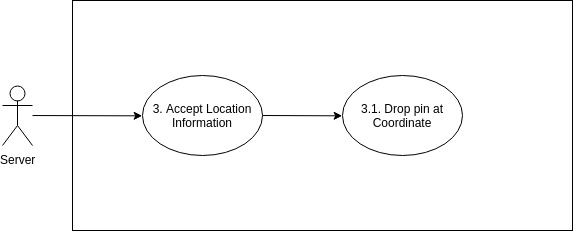
\includegraphics[scale=0.45]{./assets/images/mapping-ucd.jpg}
				\label{fig: object-recognition-ucd }
				\caption{Mapping Use Case Diagram}
			\end{figure}

		\end{flushleft}
	\end{center}
